\chapter{Übersichtskalender}\label{kalender}
Der in Abbildung~\ref{fig:kalender} gezeigte Kalender ist das Startfenster des Programms.
In ihm werden die Fahrtage und Aktivitäten des ausgwählten Monats angezeigt.
Ebenso enthält eine Liste auf der rechten Seite alle Aktivitäten nach Datum sortiert.
Jeder Eintrag kann durch einen Doppelklick geöffnet werden.

\begin{figure}[h!]
  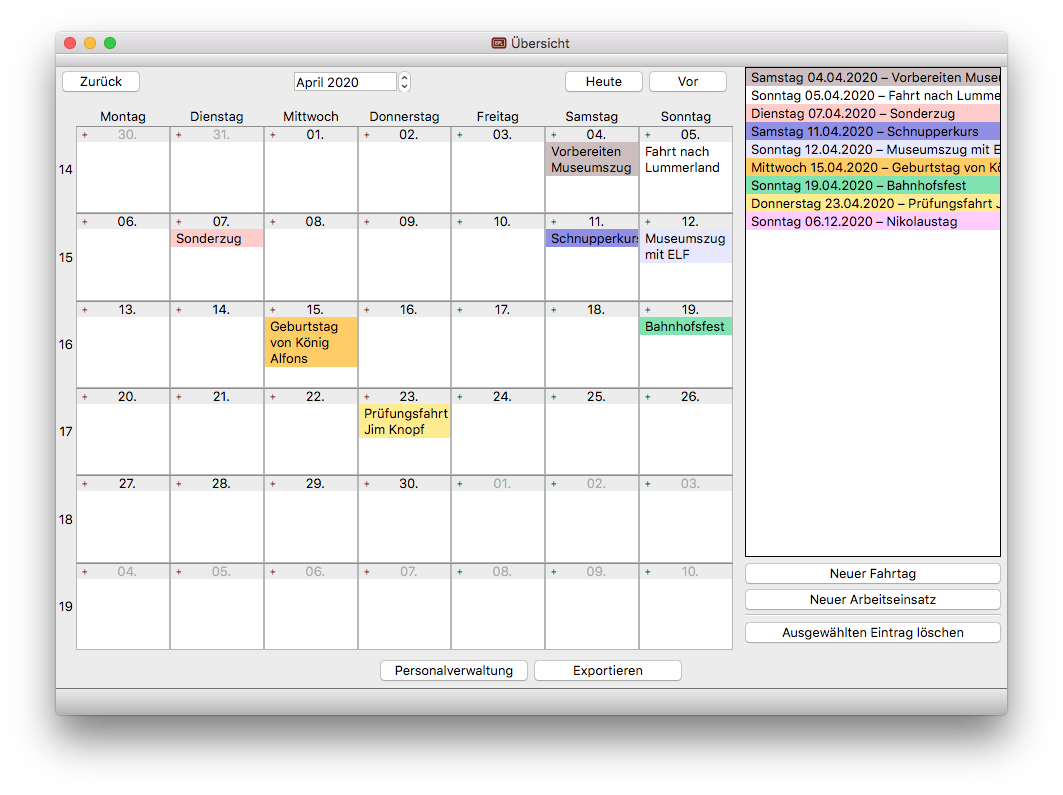
\includegraphics[width=\textwidth]{img/kalender}
  \caption{Der Kalender mit den eingetragenen Fahrtagen und Arbeitseinsätzen}
  \label{fig:kalender}
\end{figure}



\section{Anlegen von Aktivitäten}\label{kalender:anlegen}
\paragraph{Fahrtag}
Um einen neuen Fahrtag anzulegen, klicken Sie auf den Knopf "`Neuer Fahrtag"'.
Es wird ein Fahrtag mit dem aktuellen Datum angelegt und das entsprechende Fenster geöffnet (sieh Kapitel~\ref{fahrtag})
Die Fahrtage werden, um einen schnelleren Überblick zu bekommen, in verschiedenen Farben anhand ihrer Art eingefärbt.

\paragraph{Arbeitseinsatz}
Ein neuer Arbeitseinsatz kann mit Hilfe des Knopfes "`Neuer Arbeitseinsatz"' angelegt werden.
Ein Arbeitseinsatz kann auch direkt im Kalender mit einen Klick auf ``+'' mit dem entsprechenden Datum erstellt werden.
In beiden Fällen öfnet sich danach das Fenster für den Arbeitseinsatz (siehe Kapitel~\ref{arbeitseinsatz}).




\section{Löschen von Aktivitäten}\label{kalender:löschen}
Um eine Aktivität zu löschen, wählen Sie diese in der Liste aus und klicken auf den Knopf "`Ausgewählten Eintrag löschen"'.
Nach einer Sicherheitsabfrage wird der Eintrag gelöscht und verschwindet dann auch aus dem Kalender.



\section{Navigation im Kalender}\label{kalender:navigieren}
Mit den Knöpfen "`Zurück"', "`Vor"' und "`Heute"' können Sie duch den Kalender navigieren.
Ebenso können sie über das Feld auch direkt ein Datum eingeben.



\section{Exportieren von Objekten}
Um Objekte zu exportieren, klicken Sie entweder auf den Knopf "`Exportieren"' oder wählen im Datei-Menü den entsprechenden Eintrag.
Diese Funktion ist auch über den Tastaturbefehl \cmnd{cmd+P} beziehungsweise \cmnd{ctrl+P} zu erreichen.
Weitere Informationen finden Sie in Kapitel~\ref{export:aktivitaeten}.



\section{Das Datei-Menü}
Im Datei-Menü stehen Ihnen folgende Funktionen zur Verfügung:
\begin{description}
  \item[Neu]
  Erstellt ein neues Fenster mit einer leeren Einsatzplaner-Instanz.

  \item[Öffnen \dots]
  Es wird ein Dialog geöffnet, mit dem eine \texttt{.ako}-Datei geöffnet werden kann.

  \item[Zuletzt benutzt]
  Unter diesem Eintrag finden Sie die füf zuletzt verwendeten Dateien.
  Sie können direkt geöffnet werden.
  Ebenso können Sie bei Bedarf die Liste leeren.

  \item[Speichern]
  Die Datei wird an dem bisher bekannten Pfad gesichert, oder Sie werden nach einem Ort zum Sichern der Datei gefragt.

  \item[Sichern unter \dots]
  Sie können einen Ort auswählen, an dem die Datei gespeichert werden soll.
  Zur automatischen Speicherung der Daten finden Sie in Kapitel~\ref{einstellungen} weitere Informationen.

  \item[Stammdaten sichern unter \dots]
  Diese Funktion bietet die Möglichkeit, die unveränderlichen Personaldaten zu exportieren.
  Ebenso werden die Datei-Einstellungen übernommen.
  Es werden somit keine Fahrtage oder Arbeitseinsätze gespeichert.
  Diese Funktion dupliziert sozusagen die aktuelle Datei und löscht dabei alle Fahrtage und Arbeitseinsätze.


  \item[Eigenschaften]
  Hier können Sie das Online-Tool aktivieren und konfigurieren.
  Weitere Informationen in Kapitel~\ref{upload}.

  \item[Schließen]
  Schließt das aktuelle Fenster.
  Bei ungesicherten Veränderungen wird vor dem Schließen nachgefragt, ob die Änderungen gespeichert werden sollen.
  Wenn kein Fenster mehr geöffnet ist, wird das Programm beendet.

  \item[Exportieren \dots]
  Ruft die Exportfunktion auf.
  Weitere Funktionen in Kapitel \ref{export}.
\end{description}
